\section{Python Simulation}

Running the simulation in its base form, with all parameters unchanged and as stated in table~\ref{tab:sim_parameters} produces the graph in figure~\ref{fig:sim default}. The pink line represents the power draw from the drone, this illustrates most clearly what phase of the mission is currently happening. Takeoff happens around half an hour into the simulation, then a 1 hour climb with high power demand after which the drone cruises for the rest of the mission, using less power. As a range was given for both climb and cruise power the simulation picks a random value in the range each timestep, hence this line appears very thick.

The red line represents the content of the battery. It starts empty and begins to charge, when it is at 50\% the drone starts liftoff. This uses more power than the fuel cell can provide, therefore the battery supplies the additional power and thus discharges over time. When the drone switches to cruising the battery can charge again slowly. Note how the battery discharges rapidly around the 14 hour mark. This is because the CGG has run out (indicated by the yellow line) and the fuel cell can no longer provide any power. At this point, all the power is delivered by the battery until it is at 10\%, then the mission is at an end or a new CGG is ignited in case multiple CGG's were brought on the mission.

\begin{figure}[htp]
    \centering
    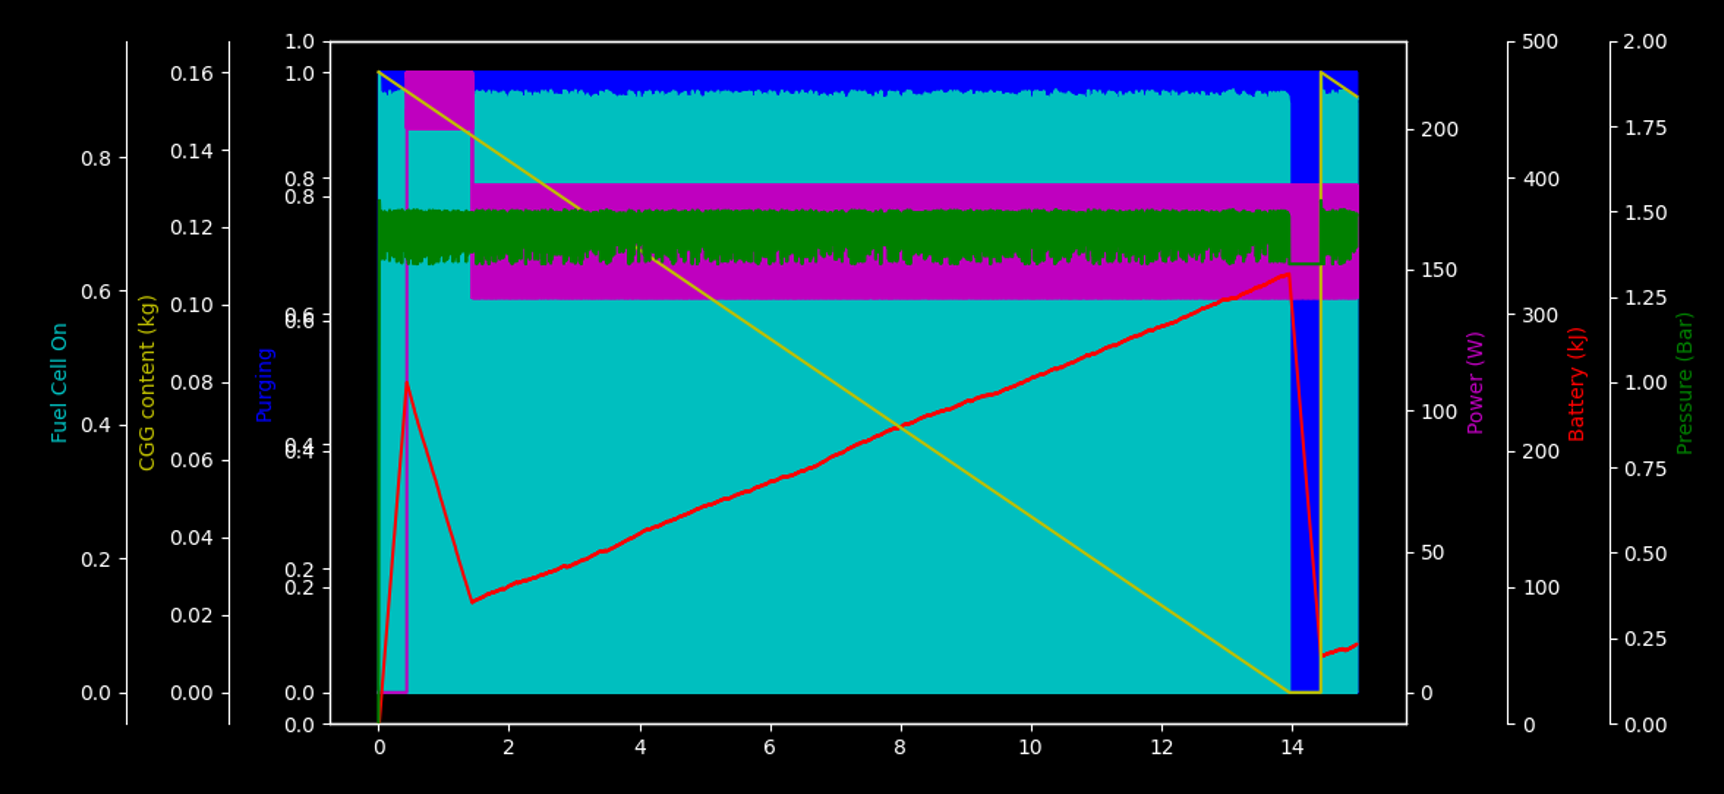
\includegraphics[width=\textwidth]{media/sim/default.png}
    \caption{Simulation Result}
    \label{fig:sim default}
\end{figure}

The green, blue and cyan lines indicate pressure in the buffer volume, whether a purge event is happening and how much power the fuel cell produces respectively. At the scale of figure~\ref{fig:sim default} their behaviour is poorly visible. Figure~\ref{fig:sim purge} provides a zoomed in view around the moment that a purge event is happening, there the behaviour of the three lines is better visible. Note however, that some lines have been excluded from this view and the scales have been altered for better visibility.

The blue line is at zero when no purge event is happening and jumps to one during a purge event. In the middle of the graph a purge event of around two seconds is visible. During the purge event the fuel cell uses hydrogen at an increased rate. Consequently, the pressure in the buffer volume drops to supply this extra hydrogen which can be seen in the green line. The controller notices this pressure drop and limits the power output of the fuel cell thereby limiting the hydrogen consumption, this can be seen by the cyan line dropping to zero.

After the purge event, the fuel cell is still limited, allowing the pressure in the buffer volume to build up again. When this pressure has been largely recovered, the fuel cell is allowed to produce power again. The reduction in power output from the fuel cell is compensated by the battery, which is visible in the red line.

\begin{figure}[htp]
    \centering
    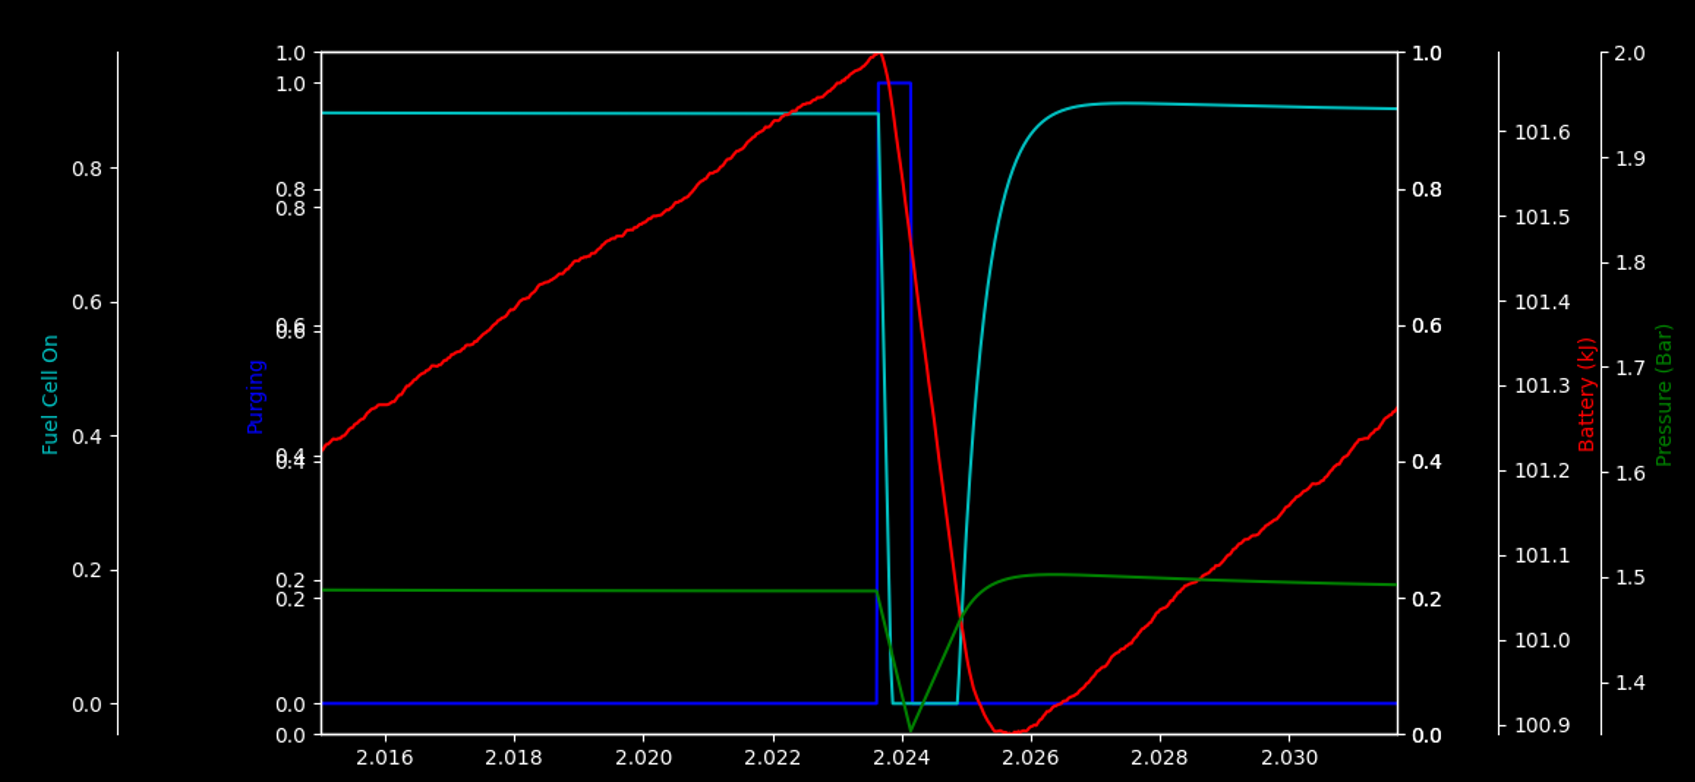
\includegraphics[width=\textwidth]{media/sim/purge.png}
    \caption{Purge Event}
    \label{fig:sim purge}
\end{figure}

\newpage
% Many of the parameters used in this simulation were altered to investigate their effect on the overall system behaviour. These results were used during the design of the hydrogen power system, and as such will be discussed further in chapter~\ref{sec:air design}.

The simulation results will also need to be verified against real-world test results. For this and other purposes the compressed air equivalent system was developed that will perform the gas flow of the hydrogen power system but with compressed air instead of hydrogen. Section~\ref{sec:air results} will compare the results from the simulation with the compressed air equivalent system.

% \todo{Results with different parameters}
The simulation can also be run with different parameters. Figure~\ref{fig:1cgg low} and~\ref{fig:1cgg high} show the simulation results with the average cruise power set to the lower and upper bound respectively. There can be seen that when the power consumption is high, the fuel cell is just capable of charging the battery. When the power consumption is low however, the battery must charge faster to absorb the excess electricity, which results in it being fully charged after about five hours. Excess hydrogen then builds pressure in the buffer volume quickly and eventually escapes through the pressure relief valve. 18.5 grams of hydrogen was vented and thus not used to generate power.

Figure~\ref{fig:4cgg low} shows the same lower limit but with four CGG's containing a quarter of the hydrogen each. This allows the battery to discharge after a CGG runs out, preventing this wasted hydrogen. Consequently the flight with four CGGs lasted over 15 hours, compared to less than 14 with only one CGG.

Cruise power and CGG amount are only two of the many configurable parameters listed in table~\ref{tab:sim_parameters}. The configurability of this simulation allows it to also be used in architecture design choices for the larger SHARP project.
\begin{figure}[htp]
    \begin{subfigure}{\textwidth}
        \centering
        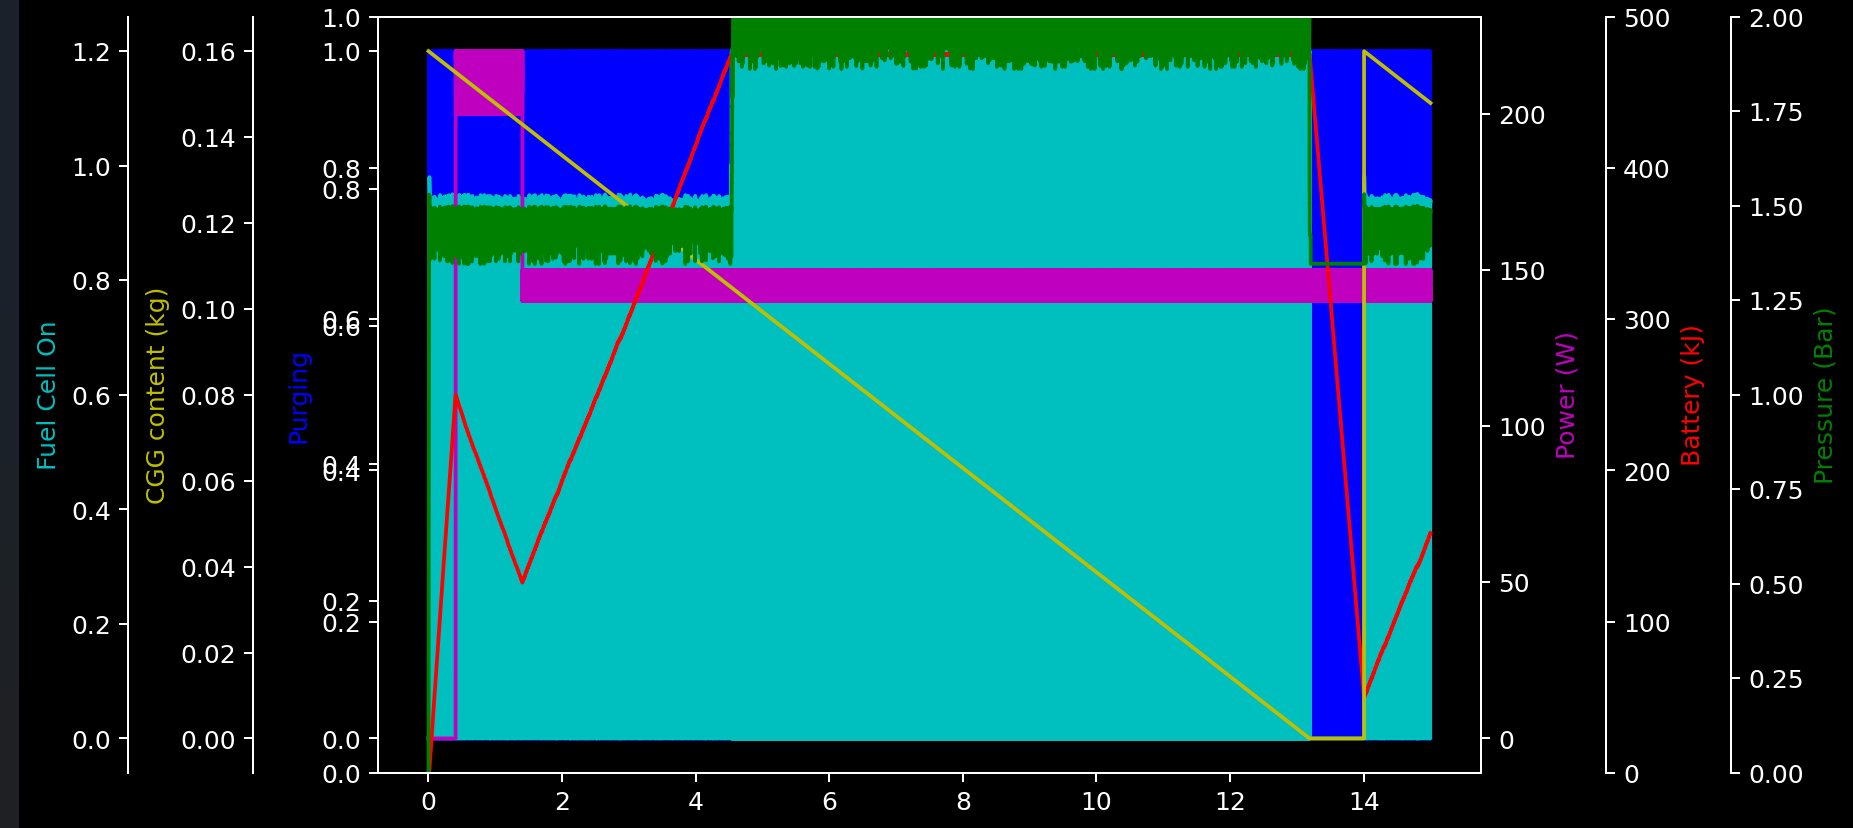
\includegraphics[width=\textwidth]{media/sim/1cgg low.png}
        \caption{Simulation with 1 CGG and 145 W cruise power}
        \label{fig:1cgg low}
    \end{subfigure}
    \begin{subfigure}{\textwidth}
        \centering
        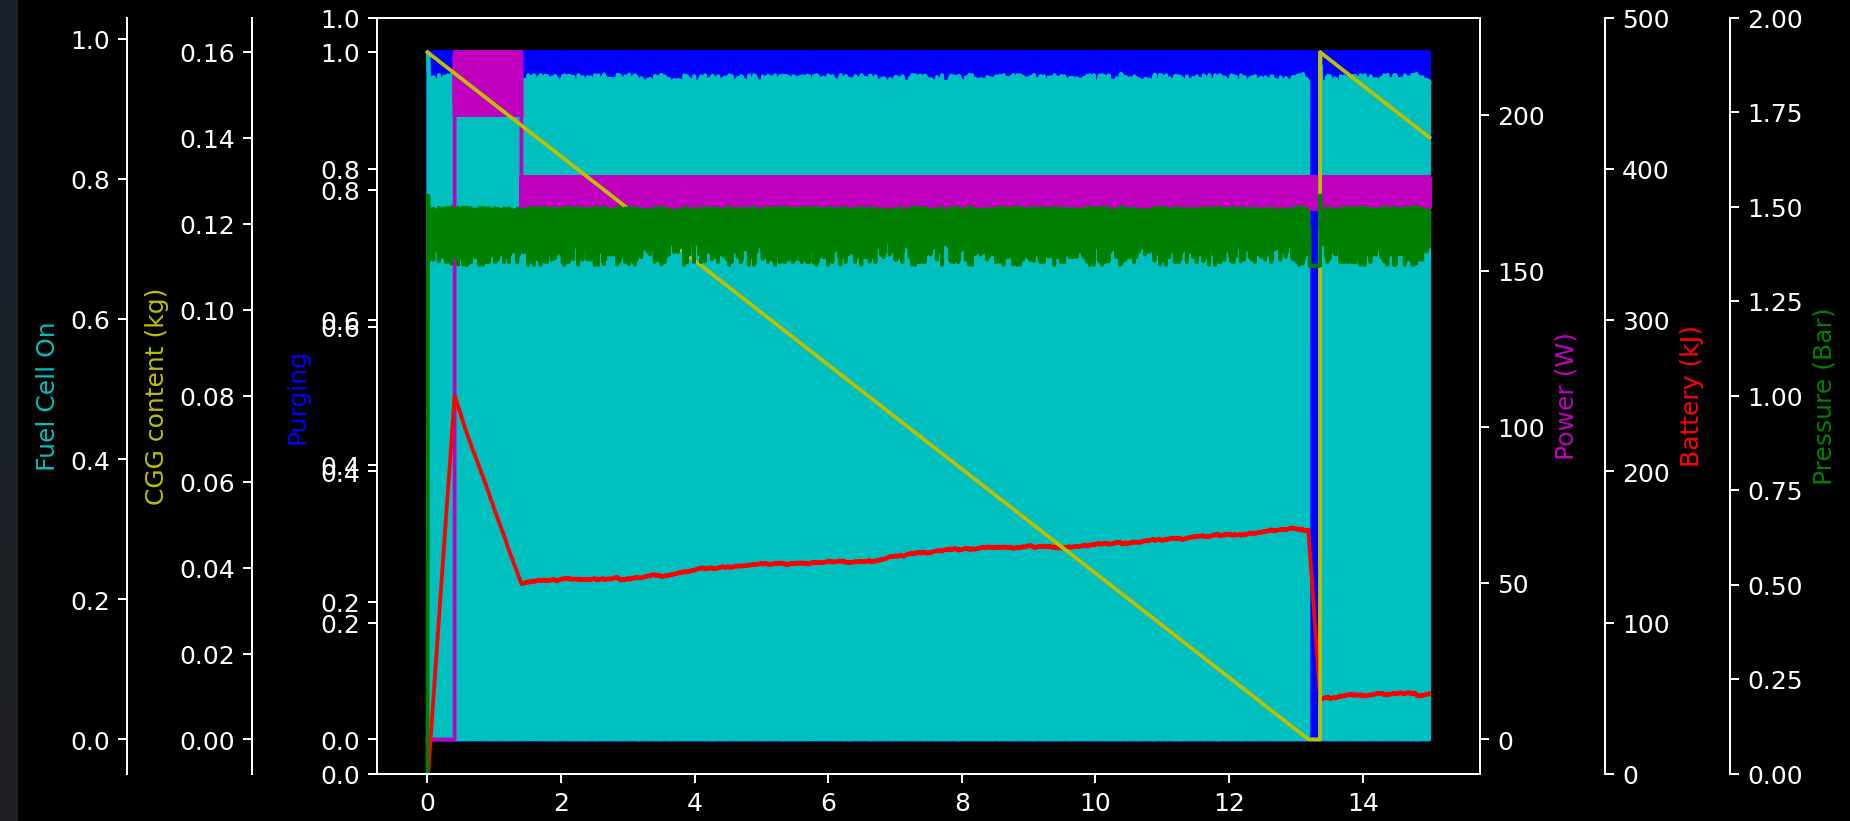
\includegraphics[width=\textwidth]{media/sim/1cgg high.png}
        \caption{Simulation with 1 CGG and 175 W cruise power}
        \label{fig:1cgg high}
    \end{subfigure}
    \begin{subfigure}{\textwidth}
        \centering
        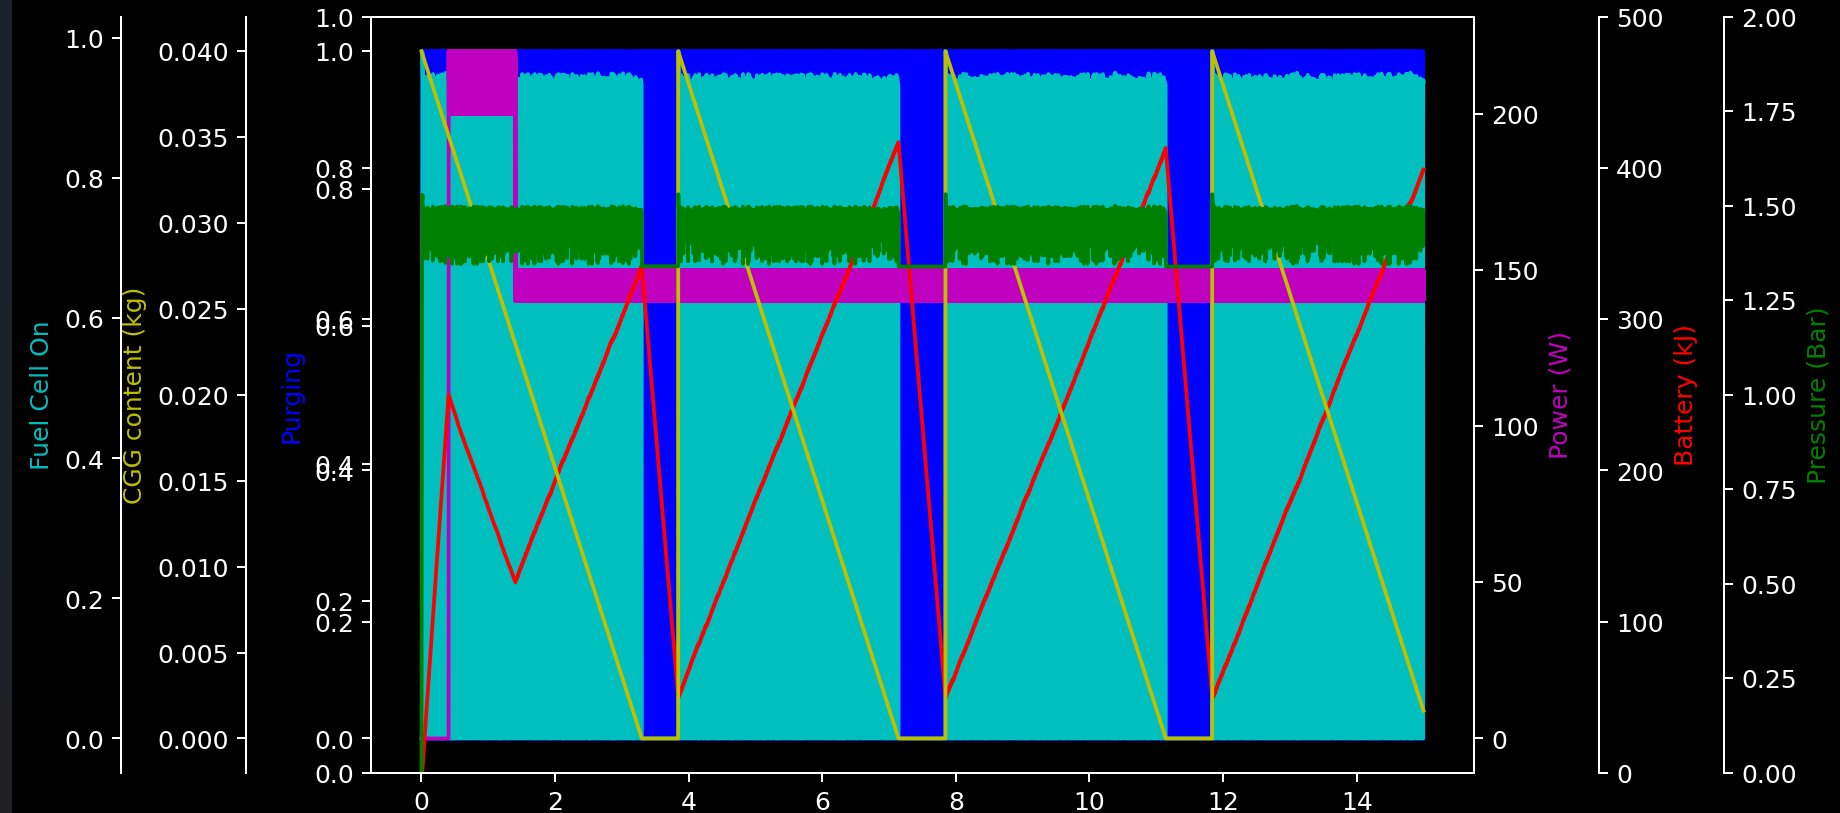
\includegraphics[width=\textwidth]{media/sim/4cgg low.png}
        \caption{Simulation with 4 CGG and 145 W cruise power}
        \label{fig:4cgg low}
    \end{subfigure}
    \caption{Simulation with different parameters}
    \label{fig:sim parameter results}
\end{figure}

% \begin{figure}[htp]
%     \centering
%     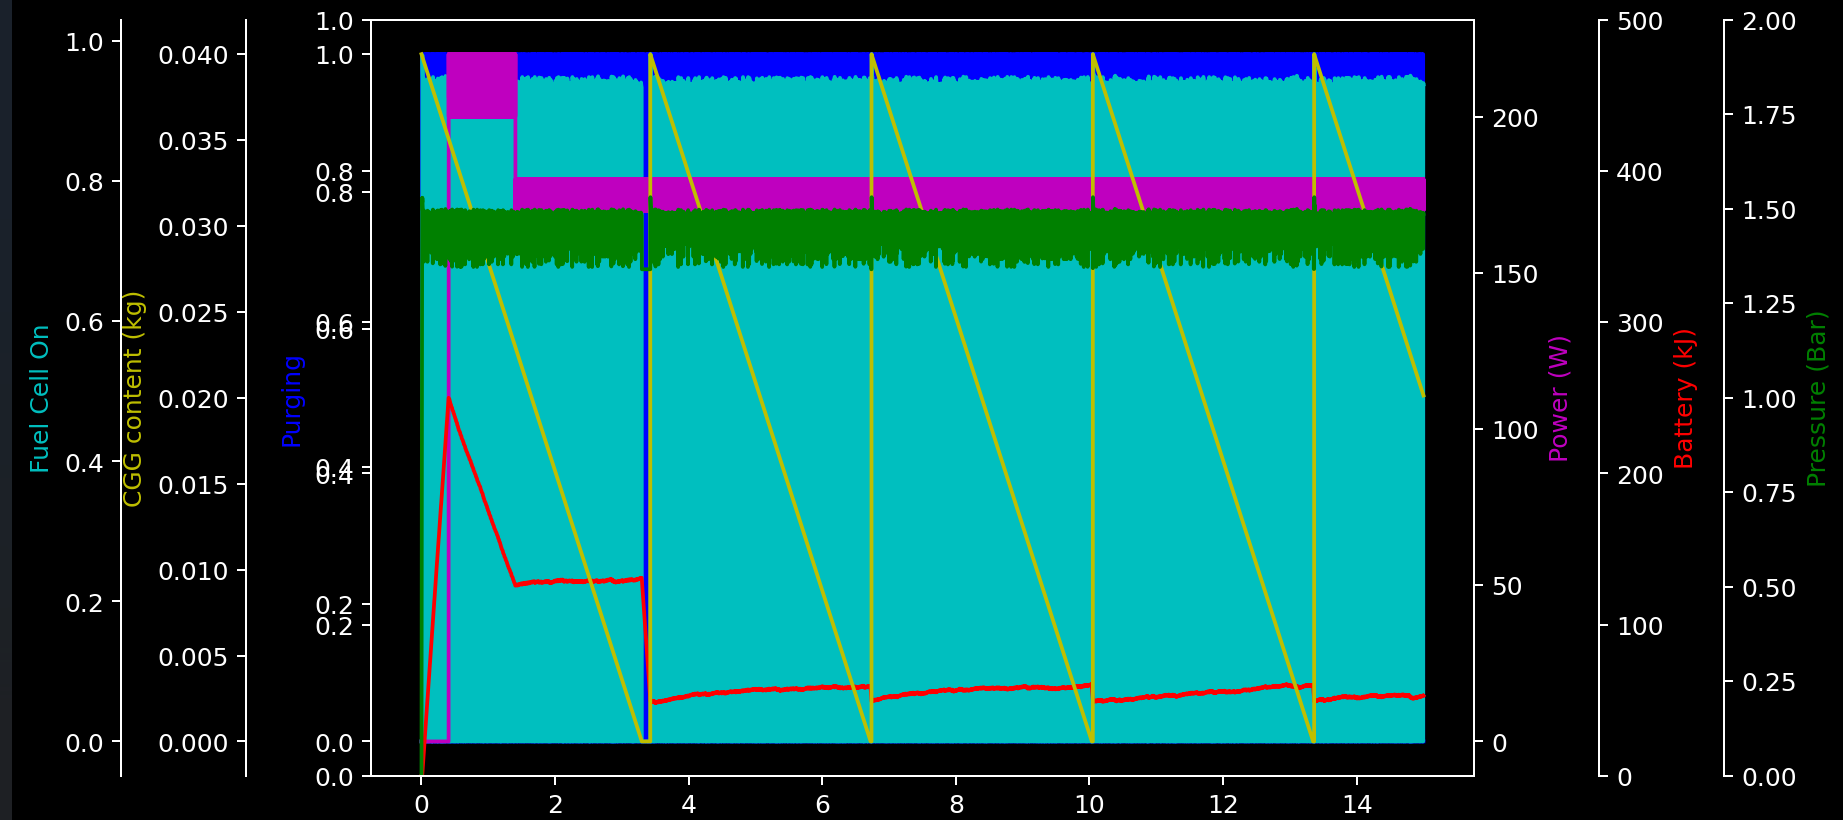
\includegraphics[width=\textwidth]{media/sim/4cgg high.png}
%     \caption{Simulation with 4 CGG and 175 W cruise power}
%     \label{fig:4cgg high}
% \end{figure}
\newpage
